% ============================================================================
% ICASSP 2027 submission -- FieldGraph-Net
% Built from 婵炴潙鍚嬫穱娲敊閸涙潙鍐€闁绘挸娴风涵鈧柣鐔告磻閻掞箓鎯?ICASSP2027_Paper_Templates/Template.tex (spconf.sty).
% Style files in this directory: spconf.sty, IEEEbib.bst, strings.bib.
% Bibliography: refs.bib (exactly 20 entries, keys stable).
%
% STATUS: SKELETON ONLY. Section bodies are intentionally empty and marked TODO;
% they are written one section at a time, not generated in a single pass.
% Author names and affiliation are deliberately left blank (to be supplied).
%
% Layout budget (per author requirements):
%   abstract        <= 200 words
%   Introduction    template length
%   Method          must end before the middle of page 3
%   Experiments     <= 1.5 pages
%   Exp. Settings   <= 300 words
%   Conclusion      within page 4, <= 200 words
%   References      20
% Writing constraints: no em-dashes; do not overuse hyphens.
% ============================================================================
\documentclass{article}
\usepackage{spconf,amsmath,graphicx,hyperref}
\def\x{{\mathbf x}}
\def\L{{\cal L}}

% Title.
\title{\textbf{FieldGraph-Net: Protocol-Guided Network Intrusion Detection with Structural Analysis}}
%
% Authors and affiliation left blank on purpose (to be supplied by the author).
% Single address.
% ---------------

\name{Lei Zhu$^{1}$, Lixin Luo$^{1}$$^*$, Ruinan Peng$^{1}$$^*$\thanks{$^*$ Corresponding author:  3240913007@stu.xaut.edu.cn, 1231211009@stu.xaut.edu.cn}, Kun Jiang$^{1}$, Qindong Sun$^{2}$, Yichuan Wang$^{1}$, Jie Zhang$^{1}$, Zheng Liu$^{1}$}
\address{$^{1}$Xi'an University of Technology, China; $^{2}$Xi'an Jiaotong University, China}

\begin{document}
\ninept
\maketitle

\begin{abstract}
Network intrusion detection must accommodate traffic from protocols absent during
classifier training. We introduce FieldGraph-Net, a structural front end that uses
predicted protocol identity to guide flow analysis. Message segmentation yields
candidate fields used to construct a structural fingerprint with 24 components and
a heterogeneous field graph. A graph classifier predicts protocol identity from
the field graph, using protocol labels for supervision. The router sends flows
assigned to the attack classifier's training protocol domain to that classifier
and directs the remainder to structural clustering. A decision rule combines
classifier alerts with structural risk indicators. On CIC IoT 2023, thresholds are
selected from benign scores in the evaluation set to obtain realized false
positive rates near 20\%. Across five attack categories, FieldGraph-Net achieves a
mean F1 of 0.5076, compared with 0.4323 for maximum softmax probability, the
strongest baseline by mean F1. Baseline results are averaged over five seeds;
FieldGraph-Net contributes one operating point per category. The framework extends
analysis coverage beyond the attack classifier's protocol domain and achieves the
highest mean F1 among the evaluated methods.
\end{abstract}

\begin{keywords}
Network intrusion detection, protocol identification, heterogeneous graph neural networks, structural fingerprinting, structural clustering
\end{keywords}

\section{Introduction}
\label{sec:intro}

Graph neural networks (GNNs) are widely used for network intrusion
detection~\cite{farrukh2023xgnid,zhou2020gnn,lo2022egraphsage}. Their deployment often
assumes that the protocol distribution observed during training remains
representative~\cite{khraisat2019survey}. Campus and industrial networks challenge
this assumption as services and protocol mixtures change over time. A classifier
can still assign a confident attack label to a flow from an unfamiliar protocol.
Identifying whether that protocol belongs to the classifier's training domain is
therefore a distinct step in assessing its prediction.

Existing approaches address different parts of this problem. Retraining requires
examples from the new setting, while learning from positive and unlabeled data
requires an observed positive class~\cite{elkan2008learning}. Open set classifiers
provide a rejection mechanism for unknown attacks~\cite{farrukh2023openset}.
Out-of-distribution (OOD) detectors use maximum softmax probability
(MSP)~\cite{hendrycks2017msp}, calibrated confidence~\cite{liang2018odin}, or
Mahalanobis distance~\cite{lee2018mahalanobis} to assess compatibility with training
data. Distribution shifts can impair these scores in network intrusion
detection~\cite{corsini2023ood}, as discussed more broadly in anomaly
detection~\cite{ruff2021anomaly}. Local Outlier Factor~\cite{breunig2000lof} and
Isolation Forest~\cite{liu2008iforest} estimate anomalies without attack labels.
These scores quantify deviations from reference data; protocol identification
provides complementary information about the traffic being assessed.

Protocol reverse engineering extracts candidate fields from message
structure~\cite{kleber2018nemesis}, and hierarchical format inference refines this
representation~\cite{hu2026mdiplier}. Protocol clustering also groups unknown traffic
through similarities in inferred specifications~\cite{li2024protocol}. These studies
motivate using field organization to guide intrusion detection. Structural extraction
can operate without attack labels, while protocol classification can use protocol
labels to learn recurring formats. Linking the resulting identity signal to a
routing decision allows unfamiliar traffic to receive a separate structural
assessment.

We propose FieldGraph-Net to implement this separation. A structural fingerprint and
a heterogeneous field graph encode each segmented message. Field Protol GNN predicts
one of twelve protocol labels, and a domain router uses protocol identity to select
the subsequent analysis path. Flows within the attack classifier's training protocol
domain receive attack predictions. Flows outside that domain enter structural
clustering, which identifies unusual message organization and associated risk
indicators. A decision rule then assigns an explicit state to each flow.

Our contributions are summarized as follows:
\begin{itemize}
  \item We combine structural fingerprints with heterogeneous field graphs to obtain
  protocol identity using protocol supervision, without requiring attack labels for
  this stage.
  \item We introduce routing by protocol domain to combine attack classification
  with structural assessment of flows outside the classifier's training domain.
  \item We evaluate the system on CIC IoT 2023 and CICIDS2017. The comparison across
  five attack categories yields a mean F1 of 0.5076, and the ablation characterizes
  the contributions of classifier scores, structural scores and the full rule.
\end{itemize}

\begin{figure*}[t]
\centering
\IfFileExists{figures/fig_arch.png}{%
  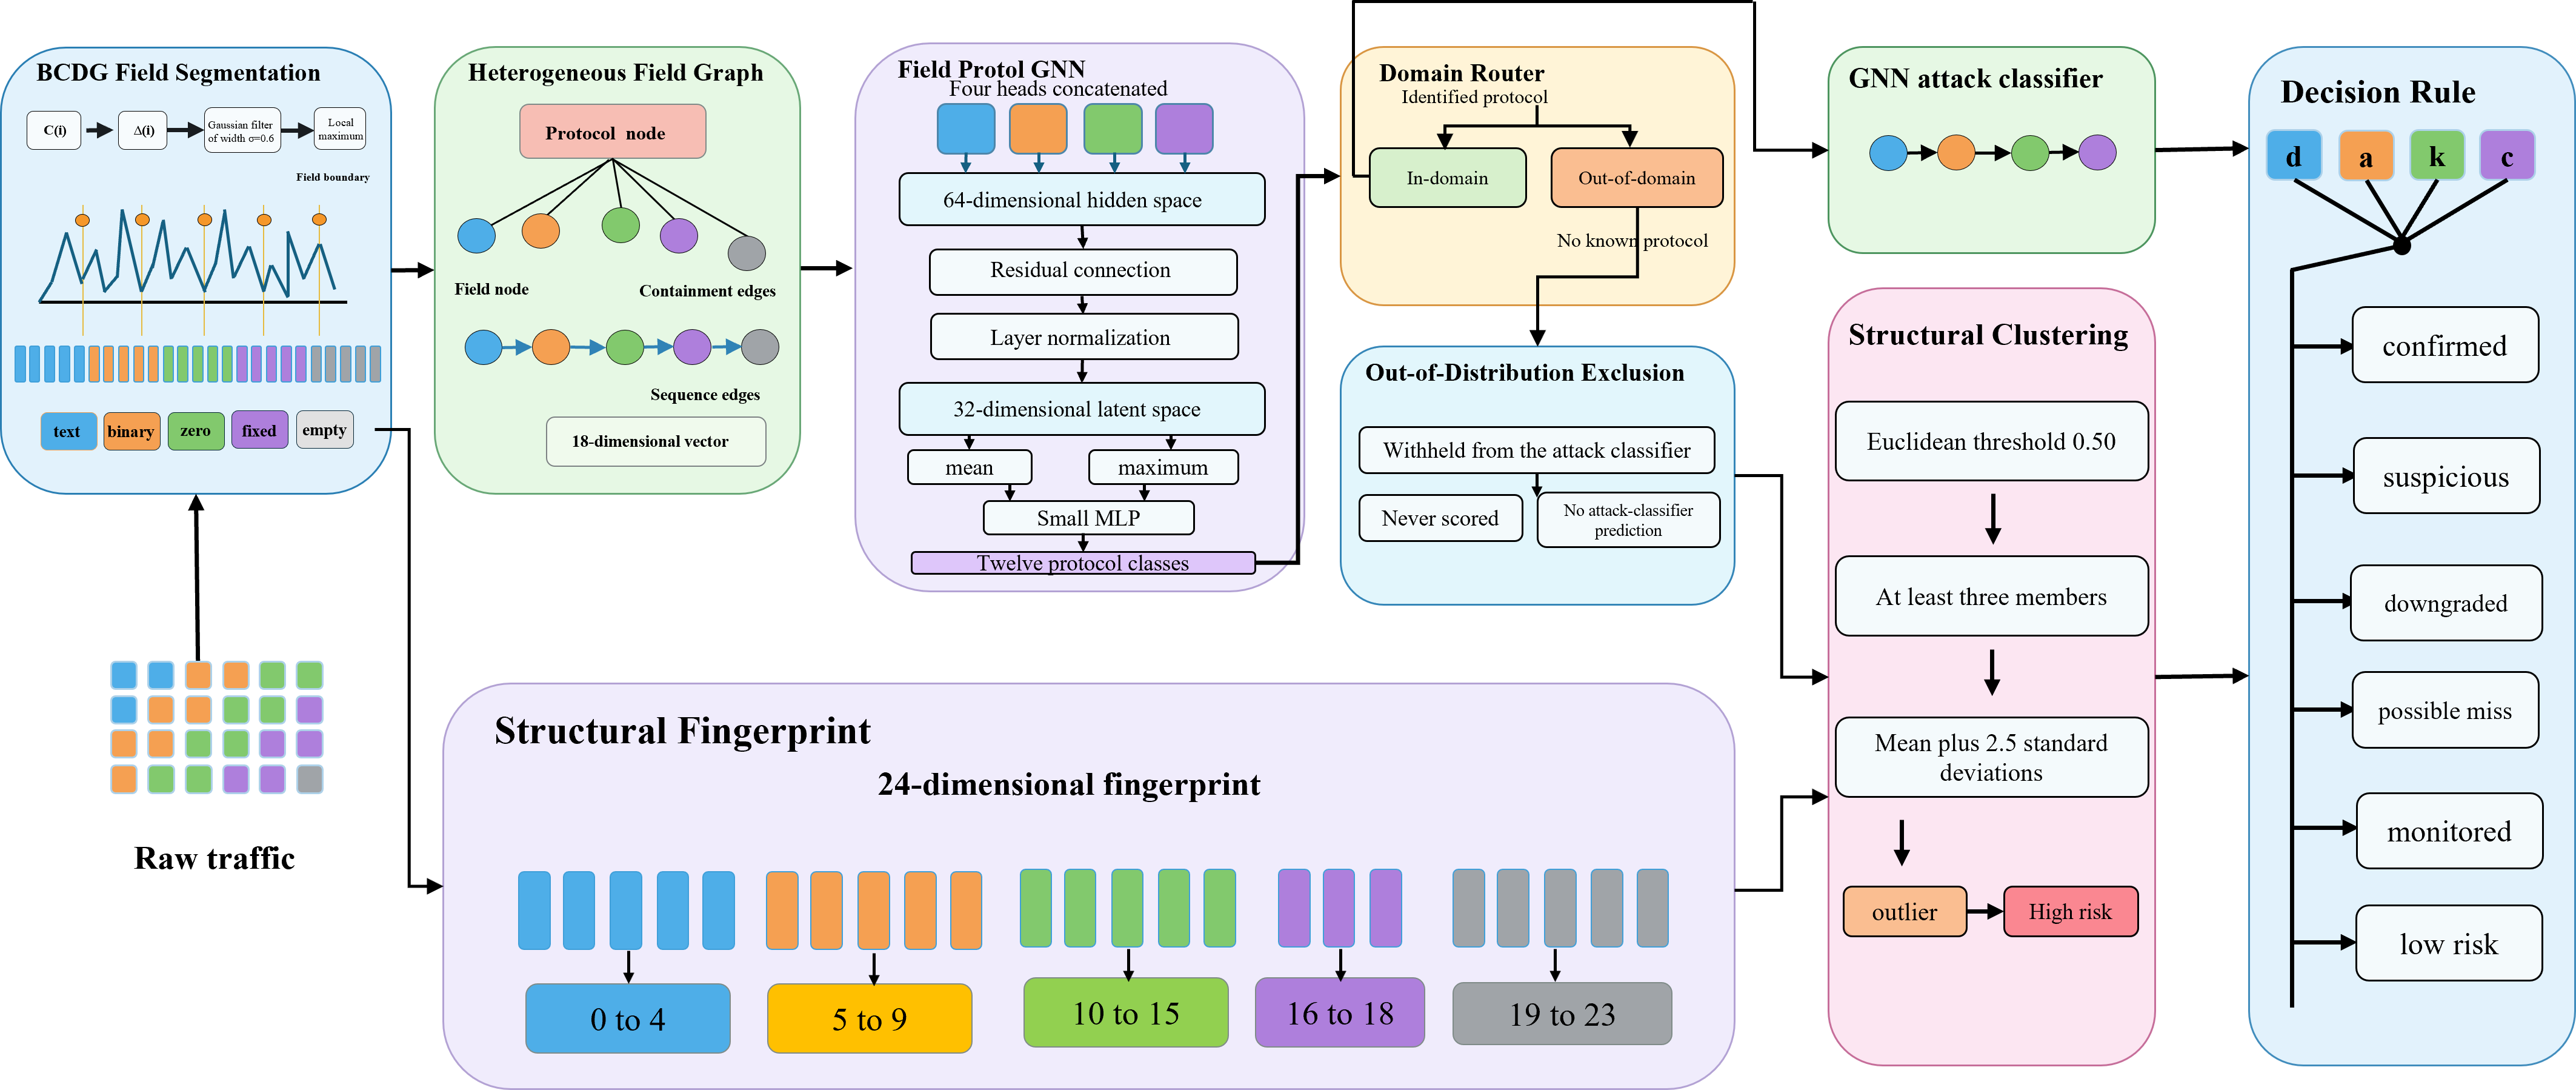
\includegraphics[width=0.95\textwidth]{figures/fig_arch}%
}{%
  \IfFileExists{figures/fig_arch.pdf}{%
    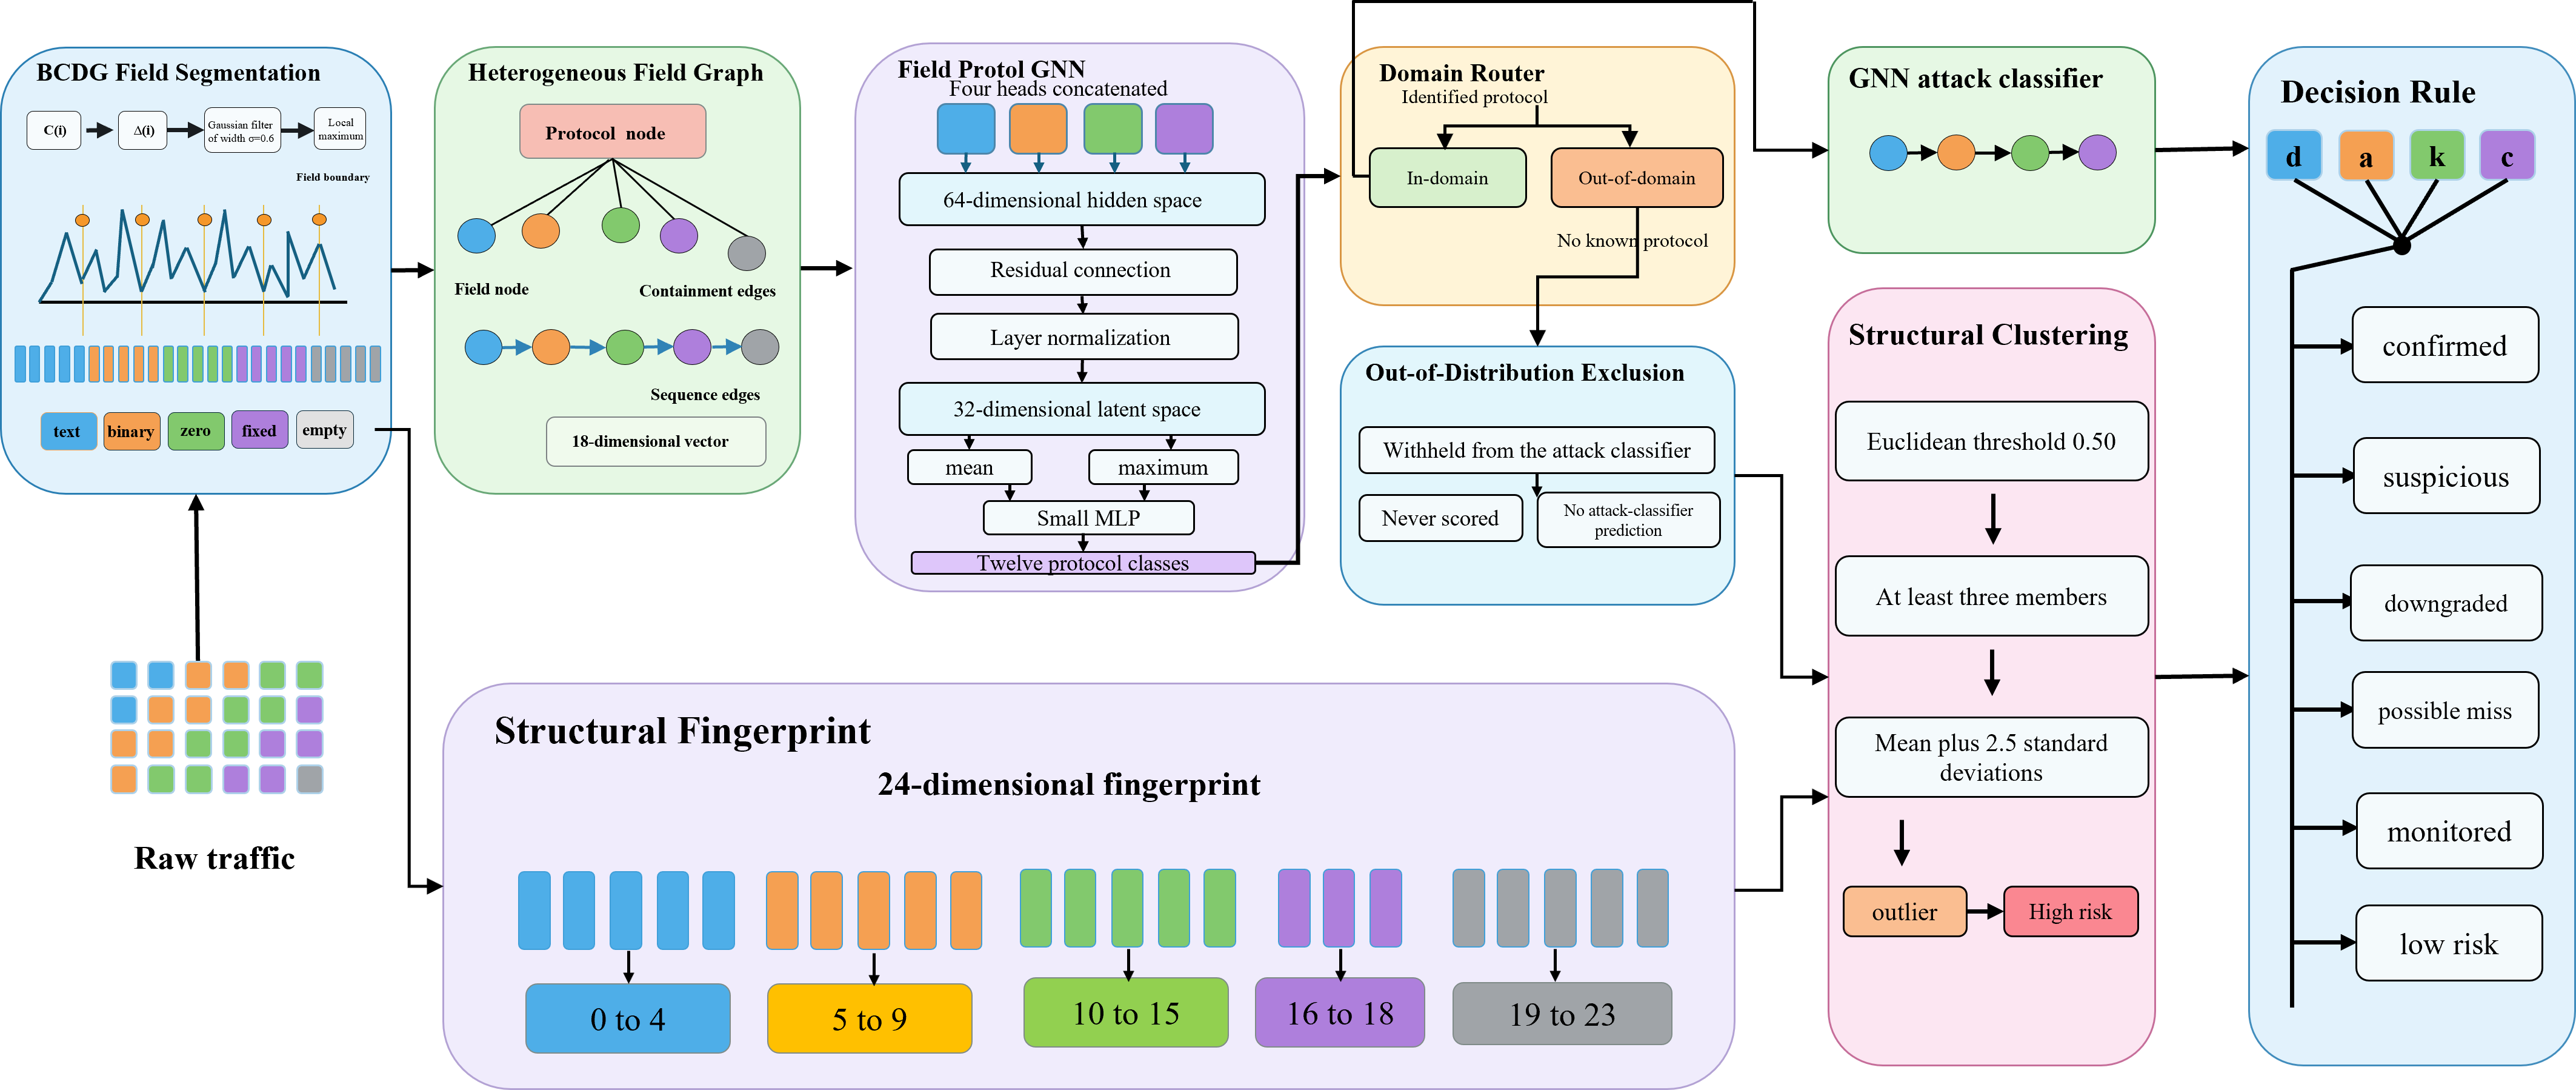
\includegraphics[width=0.95\textwidth]{figures/fig_arch}%
  }{%
    \fbox{\parbox[c][2.6cm][c]{0.94\linewidth}{\centering
      \textbf{Figure 1 placeholder}\\[2pt]
      drop \texttt{figures/fig\_arch.png} here}}%
  }%
}
\caption{Overview of FieldGraph-Net. Message segmentation supplies structural
fingerprints and heterogeneous field graphs. Field Protol GNN predicts protocol labels
for domain routing. Flows within the classifier's training protocol domain receive
attack predictions; other flows enter structural clustering. The six labels shown in
the decision interface reduce to four reachable states under the routing constraint.}
\label{fig:arch}
\end{figure*}

\section{Proposed Method}
\label{sec:method}

Figure~\ref{fig:arch} presents three stages: structural representation, protocol
identification, and routing with decision fusion. Protocol predictions assign flows
to the classifier's training protocol domain or to structural analysis; the latter
are termed OOD flows here.

\subsection{Structural Representation}
\label{ssec:repr}

\textbf{BCDG Field Segmentation.} We use Gaussian filtering of bit congruence
differences (BCDG), the structural signal introduced by
NEMESYS~\cite{kleber2018nemesis}. Bit congruence is defined as
\begin{equation}
C(i)=\frac{1}{8}\sum_{j=0}^{7}\mathbf{1}\!\left[b_i[j]=b_{i+1}[j]\right],
\quad 1\leq i<n,
\label{eq:bc}
\end{equation}
where $C(i)$ is the fraction of equal bits in adjacent bytes and
$\mathbf{1}[\cdot]$ is the indicator function. The message contains $n$ bytes;
$b_i[j]$ denotes bit $j$ of byte $i$, with bit indices from zero to seven. The indicator equals one for matching bits
and zero otherwise, so the expression averages eight comparisons. The first difference is
\mbox{$\Delta(i)=C(i+1)-C(i)$} for $1\leq i\leq n-2$, where $\Delta(i)$ measures the
change between consecutive congruences and $i$, $C$ and $n$ retain these definitions.
Gaussian smoothing uses $\sigma=0.6$, where $\sigma$ is the kernel standard
deviation in byte positions. Our local segmentation rule selects maxima of the
smoothed differences when the preceding segment contains at least two bytes. The
last segment extends to the payload boundary, and adjacent printable ASCII segments
are merged. Fields retain their offsets, lengths and implementation labels: text,
binary, zero, fixed or empty.

\textbf{Structural Fingerprint.} Each message is encoded as
$\boldsymbol{\phi}=(\phi_0,\ldots,\phi_{23})$, where $\boldsymbol{\phi}$ is the
structural fingerprint and the subscripted entries are its 24 feature components.
Components 0 to 4 describe the field count and the mean, standard deviation, minimum
and maximum field lengths. Components 5 to 9 contain the proportions of the five
field labels. Components 10 to 15 encode Shannon entropy, the distinct byte
ratio, and the first four payload bytes. Components 16 to 18 encode
the transport protocol and source and destination ports. Each port is transformed
as $q(p)=\log_2(p+1)/16$, where $p$ is an integer port number from 0 to 65535,
$q(p)$ is its normalized value, and $\log_2$ is the base two logarithm. Components
19 to 23 form a histogram of field lengths: 1, 2, 3 to 4, 5 to 8, and at least 9 bytes.

\subsection{Field Graph Protocol Identification}
\label{ssec:proto}

\textbf{Heterogeneous Field Graph.} Each graph contains one message summary node,
termed the protocol node, and one node per field. The field vector has 18 components describing offset, length, log
length, initial bytes, relative position, boundary indicators, entropy, byte diversity
and field type. The protocol node also has 18 components, summarizing message length,
field statistics, field types, entropy, byte diversity, ports and transport protocol.
Containment edges connect the protocol node to each field, and sequence edges connect
adjacent fields. Reversing both relations produces four directed relation types.

\textbf{Field Protol GNN.} Protocol classification uses two heterogeneous graph
attention layers with each four heads ~\cite{velickovic2018gat}. The update with
concatenated heads is
\begin{equation}
\mathbf{h}_v^{(\ell+1)}=
\mathop{\Vert}_{\nu=1}^{4}\rho\!\left(
\sum_{r\in\mathcal{R}_v}\sum_{u\in\mathcal{N}_r(v)}
\alpha_{vu}^{(\ell,r,\nu)}\mathbf{W}_r^{(\ell,\nu)}\mathbf{h}_u^{(\ell)}
\right),
\label{eq:gat}
\end{equation}
where $v$ is the receiving node, $u$ is a source node, and $\ell$ indexes layers.
The indices $r$ and $\nu$ denote a directed relation and an attention head,
respectively. The vectors $\mathbf{h}_u^{(\ell)}$ and
$\mathbf{h}_v^{(\ell+1)}$ are the input and output node embeddings, respectively.
The matrix $\mathbf{W}_r^{(\ell,\nu)}$ projects source embeddings for the specified
relation, layer and head. The set $\mathcal{R}_v$ contains the relations entering
$v$, and $\mathcal{N}_r(v)$ contains the corresponding source nodes. The weight
$\alpha_{vu}^{(\ell,r,\nu)}$ controls their contributions to the sums;
$\rho$ is an elementwise activation, and $\Vert$ concatenates the four heads.
The layers produce embeddings of 64 and 32 components, respectively. A residual
connection and layer normalization follow the first layer. Concatenating the
protocol node embedding with projected mean and maximum pools of field embeddings
forms the message representation. A multilayer perceptron maps this representation
to twelve protocol classes using protocol labels for supervision.

\subsection{Domain Routing and Decision Fusion}
\label{ssec:fusion}

\textbf{Domain Router.} The router compares the identified protocol with those
represented in the attack classifier's training domain. A port lookup provides a
fallback when a protocol identity is unavailable. Domain membership and protocol
recognition are distinct: a recognized protocol can still lie outside the attack
classifier's training domain.

\textbf{Out-of-Distribution Exclusion.} The router sends OOD flows to structural
analysis. The attack classifier supplies scores only for flows routed to its domain.
This separation defines the coverage of the two analysis paths.

\textbf{Structural Clustering.} Greedy clustering assigns each OOD fingerprint to
the nearest existing centroid within Euclidean distance 0.50, creating a cluster if
none qualifies. For clusters with at least three members, the outlier rule is
\begin{equation}
\delta_x=\lVert\boldsymbol{\phi}_x-\boldsymbol{\mu}_{\mathcal{C}}\rVert_2,
\qquad \delta_x>m_{\mathcal{C}}+2.5s_{\mathcal{C}},
\label{eq:outlier}
\end{equation}
where $x$ indexes a message in cluster $\mathcal{C}$ and
$\boldsymbol{\phi}_x$ denotes its structural fingerprint. The centroid
$\boldsymbol{\mu}_{\mathcal{C}}$ defines the distance $\delta_x$, and
$\lVert\cdot\rVert_2$ denotes the Euclidean norm. The quantities $m_{\mathcal{C}}$
and $s_{\mathcal{C}}$ are the mean and standard deviation of the cluster reference
distances used at scoring time. A cluster receives a high risk
flag if it contains an outlier or combines a risk indicator, such as high entropy,
with loose or moderate cohesion.

\textbf{Decision Rule.} Under domain routing, the active decision rule has four
mutually exclusive outcomes:
\begin{equation}
\Phi(d,a,k,c)=
\begin{cases}
\text{confirmed}, & d\wedge a,\\
\text{possible miss}, & \neg d\wedge\neg k\wedge c,\\
\text{monitored}, & \neg d\wedge\neg k\wedge\neg c,\\
\text{low risk}, & \text{otherwise},
\end{cases}
\label{eq:fusion}
\end{equation}
where $\Phi$ is the output state, and $\wedge$ and $\neg$ denote logical
conjunction and negation. The Boolean indicators $d$, $a$, $k$ and $c$ denote
training domain membership, a classifier attack prediction, recognized protocol
identity and a high risk cluster, respectively. Routing imposes $a\leq d$, where $a$ uses zero as a bookkeeping value
for OOD flows and $d$ retains its domain indicator meaning. Consequently,
the interface labels suspicious and downgraded are inactive because both require an
attack prediction on an OOD flow. The confirmed state denotes a classifier alert,
and possible miss denotes a structural alert for an unrecognized protocol.

\section{Experiments}
\label{sec:exp}

\subsection{Experimental Settings}
\label{ssec:settings}

\textbf{Datasets and Baselines.} The CIC IoT 2023 evaluation~\cite{neto2023ciciot}
uses 70 packet capture (PCAP) chunks containing 3233 flows. This subset includes
benign traffic and six of the base detector's seven attack output classes. Its
denial of service (DoS) class has no samples. CICIDS2017~\cite{sharafaldin2018cicids} provides a separate
evaluation corpus excluded from training. The local extractor computes the 82 flow
features specified by the GNN4ID feature pipeline~\cite{farrukh2023xgnid} directly from PCAP files. The base
detector was retrained with its reference pipeline using
NFStream~\cite{aouini2021nfstream}. Feature values and flow counts differ between
the two extraction pipelines, introducing a preprocessing difference between
training and evaluation. All compared methods use the same local extractor and
base detector. The OOD baselines are MSP~\cite{hendrycks2017msp},
ODIN~\cite{liang2018odin} with temperature calibrated on benign flows from the
training domain, and Mahalanobis scoring~\cite{lee2018mahalanobis} with class means
and shared covariance. These guards use the existing classifier and its training
information without additional attack annotations for OOD calibration.

\textbf{Metrics and Implementation.} Thresholds are selected from benign scores to
minimize the absolute difference between the realized false positive rate (FPR)
and 20\%, with ties resolved by the smaller threshold. We report recall, F1 and
FPR; the score AUC is the area under the receiver operating characteristic curve.
Table~\ref{tab:comparison} averages baseline results across five seeds and reports
one operating point per attack category for FieldGraph-Net. Evaluation uses Python
3.10.11, PyTorch 2.13.0, PyTorch Geometric 2.8.0, scikit-learn 1.7.2, NumPy 2.2.6
and SciPy 1.15.3 on an Intel Core i9-13980HX running Windows 11. Detector retraining
uses an NVIDIA RTX 4060 with PyTorch 2.13.0+cu126; evaluation runs on the CPU.

\subsection{Results and Analysis}
\label{ssec:results}

\textbf{Simulation Experiment.} Table~\ref{tab:simulation} compares alert rates
in documented CICIDS2017 attack windows with the reference rate on the same day.
All extracted flows from the selected captures were retained. Enrichment is the ratio of the window alert
rate to the corresponding reference rate, providing a temporal measure of alert
concentration. The evaluation uses the published attack schedule to define windows;
reliable alignment between the released flow labels and the locally extracted
flows was not established.

\begin{table}[h]
	\centering
	\caption{CICIDS2017 evaluation using all extracted flows. Alert rates in documented
		attack windows are compared with the reference alert rate on the same day. Enrichment is the
		ratio of these rates.}
	\label{tab:simulation}
	\footnotesize
	\setlength{\tabcolsep}{4pt}
	\begin{tabular}{@{}llrr@{}}
		\hline
		Day & Window & Alert & Enrich. \\
		\hline
		Wed & DoS Slowloris        & 0.5008 & $1.81\times$ \\
		& DoS Slowhttptest     & 0.4104 & $1.48\times$ \\
		& DoS Hulk             & 0.6882 & $2.48\times$ \\
		& DoS GoldenEye        & 0.5166 & $1.86\times$ \\
		& Heartbleed           & 0.2588 & $0.93\times$ \\
		Fri & Botnet ARES          & 0.2038 & $0.74\times$ \\
		& PortScan, rules on   & 0.2833 & $1.03\times$ \\
		& PortScan, rules off  & 0.8120 & $2.96\times$ \\
		& DDoS LOIT            & 0.0959 & $0.35\times$ \\
		\hline
		\multicolumn{2}{@{}l}{Reference, Wed / Fri} & 0.2772 / 0.2739 & $1.00\times$ \\
		\hline
	\end{tabular}
\end{table}

Five windows showed enrichment from 1.48 to 2.96 times the reference rate: Slowloris,
Slowhttptest, Hulk, GoldenEye and PortScan with firewall rules disabled. PortScan
with rules enabled yielded 1.03 times the reference rate, a small numerical increase.
Heartbleed, Botnet ARES and DDoS LOIT yielded ratios of 0.93, 0.74 and 0.35,
respectively. Thus, alert concentration varied across attack windows and firewall
conditions.

Structural clustering responds to deviations in message organization. Repeated
messages with similar structure can remain close to a cluster centroid even when
their aggregate activity is malicious. This property motivates complementary
features for traffic volume and temporal behavior. The window comparisons identify settings for examining these complementary signals.

\textbf{Comparative Experiment.} Table~\ref{tab:comparison} reports F1 for five attack
categories. FieldGraph-Net achieved the highest reported mean F1, 0.5076, compared
with 0.4323 for MSP, 0.3710 for the raw detector and 0.3287 for ODIN. The difference
from MSP was 0.0753. These means summarize performance across the listed attack
categories at the reported operating points.

\begin{table}[h]
	\centering
	\caption{F1 across five attack categories at a realized FPR near 20\%. Thresholds
		use benign scores. Baseline entries average five seeds; Ours uses one operating point
		per category.}
	\label{tab:comparison}
	\footnotesize
	\setlength{\tabcolsep}{3.2pt}
	\begin{tabular}{@{}lccccc@{}}
		\hline
		Attack & GNN-raw & MSP & ODIN & Mahal. & Ours \\
		\hline
		DNS\_Spoof          & 0.2747 & 0.3560 & 0.1667 & \textbf{0.5390} & 0.4792 \\
		Mirai               & 0.4060 & 0.4506 & 0.2873 & 0.3580 & \textbf{0.6230} \\
		SqlInjection        & 0.3519 & 0.3574 & 0.3688 & 0.4136 & \textbf{0.4226} \\
		DictBruteForce      & 0.4425 & 0.3883 & 0.2444 & 0.4465 & \textbf{0.5676} \\
		Recon-PortScan      & 0.3801 & \textbf{0.6093} & 0.5764 & 0.3831 & 0.4457 \\
		\hline
		Mean                & 0.3710 & 0.4323 & 0.3287 & 0.4280 & \textbf{0.5076} \\
		\hline
	\end{tabular}
\end{table}

Relative to the strongest baseline in each category, FieldGraph-Net improved F1 by
0.1724 on Mirai and 0.1211 on dictionary brute force. Its F1 on SQL injection was
0.4226, exceeding the strongest baseline by 0.0090. On DNS spoofing, it trailed
Mahalanobis scoring by 0.0598; on reconnaissance port scanning, it trailed MSP by
0.1636. The reported point estimates therefore favor FieldGraph-Net in three
categories and a baseline in two. 

Threshold selection uses benign observations from the evaluation set to match the
reported FPR target. The comparison therefore characterizes performance at that
operating point. An independently calibrated deployment threshold can produce a
different realized FPR. The baseline entries average five seeds, while each
FieldGraph-Net entry represents one operating point for the corresponding category.

\textbf{Ablation Experiment.} Table~\ref{tab:ablation} reports the classifier
probability (A1), structural cluster score (A3), full decision rule (A4), and a fixed
routing rule (A2). A1, A3 and A4 operate at FPRs of 0.200, 0.196 and
0.206, respectively. A2 has a single operating point, with an FPR of 0.868.

\begin{table}[h]
	\centering
	\caption{Reported ablation results for a corpus of 3233 flows. A1, A3 and A4 target
		an FPR near 20\%. A2 reports its fixed operating point. AUC is not reported for rule
		outputs.}
	\label{tab:ablation}
	\footnotesize
	\setlength{\tabcolsep}{4pt}
	\begin{tabular}{@{}lccccc@{}}
		\hline
		Variant & Score & FPR & Recall & F1 & AUC \\
		\hline
		A1 & classifier prob. & 0.200 & 0.2759 & 0.4204 & 0.6063 \\
		A3 & cluster score   & 0.196 & 0.2378 & 0.3735 & 0.4973 \\
		A4 & full rule       & 0.206 & \textbf{0.3696} & \textbf{0.5252} & n/a \\
		\hline
		A2 & fixed rule      & 0.868 & 0.8968 & 0.8726 & n/a \\
		\hline
	\end{tabular}
\end{table}

A4 recorded recall of 0.3696 and F1 of 0.5252. The corresponding A1 entries were
0.2759 and 0.4204, giving numerical differences of 0.0937 in recall and 0.1048 in
F1 at an FPR difference of 0.006. A3 recorded recall of 0.2378, F1 of 0.3735 and
AUC of 0.4973. Its score discrimination was close to the chance reference of 0.5,
while the full rule had the highest recall and F1 among the rows targeting 20\% FPR.
A2 attained recall of 0.8968 together with a substantially higher FPR of 0.868.

The evaluation pool contains 3233 flows. A1 supplies classifier scores for 984
flows, while routing sends the remaining 2249 flows to structural analysis. The full
rule combines classifier and structural information at the reported operating point.

\section{Conclusion}
\label{sec:conclusion}

FieldGraph-Net combines protocol identification, domain routing and structural
clustering for network intrusion detection. Protocol supervision provides an
identity signal without attack labels for the structural front end. Routing then
connects attack classification with a separate assessment of unfamiliar traffic.
Across five CIC IoT 2023 attack categories, the system achieved mean F1 of 0.5076,
compared with 0.4323 for MSP. The full rule recorded recall of 0.3696 and F1 of
0.5252 at an FPR of 0.206. CICIDS2017 evaluation showed that alert concentration
varies across attack windows, motivating complementary analysis of traffic volume
and timing. The results characterize how routing by protocol combines classifier predictions
with structural evidence at explicit operating points.

% \vfill\pagebreak
\clearpage
% ---------------------------------------------------------------------------
% ACKNOWLEDGEMENTS: pending the author's text. It is deliberately NOT emitted yet as
% an empty heading, because an empty one lands at the top of page 5 and ICASSP allows
% the fifth page to contain reference material only. When the text arrives, place it
% here; the gap between the end of the Conclusion (about 3.85 pages) and the start of
% the references (about 4.02) leaves roughly a third of a column, so two to three lines
% should fit on page 4. Re-measure the layout afterwards and add a page break if needed.
\section{Acknowledgment}
This research work is supported by the National Natural Science Founds of China (U2468206,62302389), Key Research and Development Program of Shaanxi Province (2022CGKC-09).

\section{Ethical Standards Statement}
Our evaluation uses existing packet captures from CIC IoT 2023 and CICIDS2017
for research on network intrusion detection. Reuse should follow dataset terms
and limit access to payloads and network identifiers that may expose sensitive
information. Protocol inference can aid both defense and reconnaissance, so use of
FieldGraph-Net should remain within explicitly authorized networks. The observed
false alarms warrant analyst review before traffic is blocked or devices are
 isolated.

\section{Open Science}
To support reproducibility, we provide an anonymized artifact package containing the source code, experimental scripts, model checkpoints, and selected aggregate results. The raw CIC IoT 2023 and CICIDS2017 captures are not included and must be obtained from their respective sources. The package is available at \href{https://anonymous.4open.science/r/FieldGraphNet-GitHub-DE83/README.md}{the anonymized artifact repository}.

% \vfill\pagebreak

% The spconf bibliography environment generates the REFERENCES heading.
% ============================================================================
% Template.tex ships "\bibliography{strings,refs}"; strings.bib contains only the
% template's fake placeholder entry (Lamp86, "Article Title", 1920). It is excluded
% here so the reference list contains exactly the 20 entries in refs.bib.
% Re-verified 2026-09-23: 19 registered DOI Handles and the official USENIX
% WOOT 18 landing page for NEMESYS; stable keys preserve citation numbering.
\bibliographystyle{IEEEbib}
\bibliography{strings,refs}

\end{document}
